%% LaTeX Beamer presentation template (requires beamer package)
%% see http://bitbucket.org/rivanvx/beamer/wiki/Home
%% idea contributed by H. Turgut Uyar
%% template based on a template by Till Tantau
%% this template is still evolving - it might differ in future releases!

\documentclass{beamer}

\mode<presentation>
{
\usetheme{CIn20131120}

%\setbeamercovered{transparent}
}

\usepackage[english]{babel}
\usepackage[utf8]{inputenc}
\usepackage[T1]{fontenc} 

% font definitions, try \usepackage{ae} instead of the following
% three lines if you don't like this look
\usepackage{mathptmx}
\usepackage[scaled=.90]{helvet}
\usepackage{courier}
\usepackage{tikz}
\usepackage{varwidth}
\usepackage{xspace}
\usepackage{verbatim}
\usepackage{environ}
\usepackage{ifthen}

\usetikzlibrary{arrows,trees,positioning,circuits.logic.US,shapes}
\tikzset{>=latex}

\DeclareGraphicsExtensions{.png,.pdf,.eps}
%\DeclareGraphicsExtensions{.png}
\graphicspath{{./images/},{./}}


\usepackage[T1]{fontenc}

\DeclareMathOperator{\doo}{d}
\DeclareMathOperator{\nibefore}{\lhd}
\DeclareMathOperator{\simultaneous}{\triangle}
\DeclareMathOperator{\ibefore}{\unlhd}
\DeclareMathOperator{\inter}{\cap}
\DeclareMathOperator{\union}{\cup}
\DeclareMathOperator{\tvar}{\mathsf{tvar}}
\DeclareMathOperator{\distinct}{\mathsf{distinct}}
\DeclareMathOperator{\set}{\mathsf{set}}
\DeclareMathOperator{\xbefore}{\rightarrow}
\DeclareMathOperator{\listt}{\mathsf{list}}
\DeclareMathOperator{\sett}{\mathsf{set}}
\DeclareMathOperator{\tformulat}{\mathsf{tformula}}
\DeclareMathOperator{\BasicEventMinLevel}{\mathsf{BasicEventMinLevel}}
\DeclareMathOperator{\RootProbability}{\mathsf{RootProbability}}
\DeclareMathOperator{\evaluateRule}{\mathsf{evaluateRule}}
\DeclareMathOperator{\minBasicEventLevel}{\mathsf{minBasicEventLevel}}
\DeclareMathOperator{\ftProbability}{\mathsf{ftProbability}}
\DeclareMathOperator{\defs}{\doteq}
\DeclareMathOperator{\concat}{@}
%\newcommand{\aaexp}[2]{^{#1}/_{#2}}
\newcommand{\aaexp}[2]{{\left[#1\right]}^{\left[#2\right]}}
\newcommand{\nominalvalue}[2]{\mathsf{N}^{#2}\left(#1\right)}
\newcommand{\failurevalue}[2]{\mathsf{#1}^{#2}}
\newcommand{\component}[1]{\mathsf{C}^{#1}}
\newcommand{\outvalue}[2]{\mathsf{#1}^{#2}}
\newcommand{\outvalueof}[1]{\rho\left(#1\right)}
\def\fba{fba}
\def\tfa{tfa}

\newcommand{\includeautosizegraphics}[1]{%
\includegraphics[height=0.8\textheight,width=\textwidth,keepaspectratio]{#1}%
}

\def\tikzoverlay{%
   \tikz[baseline,overlay]\node[every overlay node]
}

\tikzstyle{every overlay node}=[draw=black,fill=white,rounded corners,anchor=north west]

\tikzstyle{event text}=[text centered, 
  execute at begin node={\begin{varwidth}{2cm}},
  execute at end node={\end{varwidth}}
  ]
  
\tikzstyle{event}=[event text, rectangle, draw=black, fill=yellow!20, anchor=north]
%\tikzstyle{fault tree}=[edge from parent fork down, sibling distance=7cm, level distance=1.4cm, circuit logic US, growth parent anchor=south,nodes=event]
\tikzstyle{fault tree}=[circuit logic US]

\tikzstyle{level 1}=[sibling distance=7cm, level distance=1.4cm, growth parent anchor=south, nodes=event]
\tikzstyle{level 2}=[sibling distance=5cm]
\tikzstyle{level 3}=[sibling distance=5cm]
\tikzstyle{level 4}=[sibling distance=3cm]

\tikzstyle{gate}=[rotate=90, anchor=east, xshift=-1mm]
\tikzstyle{or gate}=[gate, or gate US,fill=blue!60]
\tikzstyle{and gate}=[gate, and gate US, fill=red!60]
\tikzstyle{basic}=[circle, fill=green!60, anchor=north, minimum width=0.5cm]

\tikzstyle{spare gate}=[shape=spare gate, fill=orange!40]
  
\tikzset{
  >=stealth',
  edge from parent path={(\tikzparentnode.south) -- ++(0,-0.95cm)
      -| (\tikzchildnode.north)},
  global scale/.style={
    scale=#1,
    every node/.style={scale=#1}
  }
}
\makeatletter
\pgfdeclareshape{spare gate}{
  \inheritsavedanchors[from=circle]
  \inheritanchor[from=circle]{center}
  \inheritanchor[from=circle]{north}
  \inheritanchor[from=circle]{south}
  \inheritanchor[from=circle]{east}
  \inheritanchor[from=circle]{west}
  \backgroundpath{%
      % Save radius to x
      \pgf@x=\radius
      % Radius is also containing the "minimum width" and "minimum height"
      % This ensures that even with no text the shape will be drawn.
      % Unless of course that min are set to 0pt
      % So no need to check for that
      % Save radius
      \pgfutil@tempdima=\pgf@x%

      % west triangle corner "b"
      \pgf@xb=-3\pgf@x%
      \pgf@yb=-4\pgf@x%
      % east triangle corner "c"
      \pgf@xc= 3\pgf@x%
      \pgf@yc=-4\pgf@x%

      % If text is present shift shape to center 
      % You need to shift more, but to get the idea
      \centerpoint
      \advance\pgf@xb by\pgf@x
      \advance\pgf@yb by\pgf@y
      \advance\pgf@xc by\pgf@x
      \advance\pgf@yc by\pgf@y

      % Save centerpoint in "a" (top triangle point)
      \pgf@xa=\pgf@x 
      \pgf@ya=\pgf@y

      % Below are good for debugging purposes.
      %\message{^^JTop : \the\pgf@xa,\the\pgf@ya}
      %\message{^^JWest: \the\pgf@xb,\the\pgf@yb}
      %\message{^^JEast: \the\pgf@xc,\the\pgf@yc}
      %\message{^^JCent: \the\pgf@x,\the\pgf@y}

      % draw triangle..
      \pgfpathmoveto{\pgfpoint{\pgf@xa}{\pgf@ya}}%
      \pgfpathlineto{\pgfpoint{\pgf@xb}{\pgf@yb}}%
      \pgfpathlineto{\pgfpoint{\pgf@xc}{\pgf@yc}}%
      \pgfpathclose

      % The radius of the small circles
      % Read in from option TODO
      \pgfutil@tempdimb=3pt

      % Move top triangle to head circle
      \advance\pgf@ya by.25\pgfutil@tempdimb
      % Move west triangle corner to west circle center
      \advance\pgf@xb by 1.5\pgfutil@tempdima
      \advance\pgf@yb by -\pgfutil@tempdimb
      % For handling line thickness if you wish "edge touch" and not "overlap"
      %\advance\pgf@yb by -.5\pgflinewidth 
      % Move east triangle corner to east circle center
      \advance\pgf@xc by-1.5\pgfutil@tempdima
      \advance\pgf@yc by -\pgfutil@tempdimb
      % For handling line thickness if you wish "edge touch" and not "overlap"
      %\advance\pgf@yc by -.5\pgflinewidth

      % This saves underlying "stuff" when you have the explicit `\pgfqpoint` and is thus a little faster
      \edef\pgf@marshal{%
          \noexpand\pgfpathcircle{%
              \noexpand\pgfqpoint{\the\pgf@xa}{\the\pgf@ya}}
          {\the\pgfutil@tempdimb}%
          \noexpand\pgfpathcircle{%
              \noexpand\pgfqpoint{\the\pgf@xb}{\the\pgf@yb}}
          {\the\pgfutil@tempdimb}%
          \noexpand\pgfpathcircle{%
              \noexpand\pgfqpoint{\the\pgf@xc}{\the\pgf@yc}}
          {\the\pgfutil@tempdimb}%
      }\pgf@marshal
  }
}
\makeatother

\def\CSPM{CSP$_M$\xspace}


\newenvironment{snippetcspm}[1][2]
{
\ifthenelse{\equal{#1}{0}}
    {\tiny}
    {
    \ifthenelse{\equal{#1}{1}}
        {\scriptsize}
        {
        \ifthenelse{\equal{#1}{2}}
            {\footnotesize}
            {\small}
        }
    }
%\begin{samepage}
\verbatim
}
{
\endverbatim
%\end{samepage}
}




\title{Fault Tree Analysis with Temporal Faults Algebra}
\subtitle{A formal approach to verify safety requirements}

%\subtitle{}

% - Use the \inst{?} command only if the authors have different
%   affiliation.
%\author{F.~Author\inst{1} \and S.~Another\inst{2}}
\author{André Didier}

% - Use the \inst command only if there are several affiliations.
% - Keep it simple, no one is interested in your street address.


\date{11 May 2015}


% This is only inserted into the PDF information catalog. Can be left
% out.
\subject{Talks}



% If you have a file called "university-logo-filename.xxx", where xxx
% is a graphic format that can be processed by latex or pdflatex,
% resp., then you can add a logo as follows:

% \pgfdeclareimage[height=0.5cm]{university-logo}{university-logo-filename}
% \logo{\pgfuseimage{university-logo}}



% Delete this, if you do not want the table of contents to pop up at
% the beginning of each subsection:
% \AtBeginSubsection[]
% {
% \begin{frame}<beamer>
% \frametitle{Outline}
% \tableofcontents[currentsection,currentsubsection]
% \end{frame}
% }

% If you wish to uncover everything in a step-wise fashion, uncomment
% the following command:

%\beamerdefaultoverlayspecification{<+->}

\begin{document}

\begin{frame}
\titlepage
\end{frame}

\begin{frame}
\frametitle{A safety problem\ldots}
\begin{enumerate}
  \item Analyse \alert<4>{large} Dynamic Fault Trees (DFT)\\
    \begin{minipage}[c]{4.60cm}
        \begin{itemize}
          \item Static Fault Tree (SFT) 
          \item Temporal Fault Trees (TFT)
          \item DFT analysis 
        \end{itemize}
    \end{minipage}
    \begin{minipage}[c]{5.3cm}
    \only<2->{$\implies$ Does the system meet safety requirements?}
    \end{minipage}
  \item Formalise DFT qualitative and quantitative analysis
    \begin{itemize}
      \item<3-> Is the analysis reliable?
      \item<3-> Does the tree represent the system model?
    \end{itemize}
\end{enumerate}
\end{frame}

%\begin{frame}{[Simple] Overview}
%\includeautosizegraphics{SimpleStrategyOverview}
%\end{frame}

%\begin{frame}<1>[label=zooms]
%\frametitle<1>{Overview}
\begin{frame}[fragile]{Overview}
\includeautosizegraphics{StrategyOverview}
\framezoom<1><2>(0cm, 0.58cm)(4.6cm, 4.1cm)
\framezoom<1><3>(3.0cm, 4.1cm)(1.8cm, 2.2cm)
\framezoom<1><4>(1.15cm, 4.85cm)(1.7cm, 2.2cm)
\framezoom<1><5>(1.7cm, 0.42cm)(3.5cm, 3.4cm)
\end{frame}
%\againframe<2->[plain]{zooms}

\begin{frame}
\frametitle{Concepts in this presentation}

\begin{itemize}
  \item \alert<2>{Systems modelling with Simulink}
  \item \alert<2>{Faults injection}
  \item \alert<2>{Faults traces}
  \item Fault Trees -- \alert<2>{Static}, Temporal and Dynamic
  \item Free Boolean Algebra
  \item Lists lattice
  \item Temporal Faults Algebra
  \item Fault modelling and safety design patterns
  \item Activation Algebra and Predicates
  \item Safety requirements and fault tree acceptance criteria
\end{itemize}

\onslide<2>{\tikzoverlay[text width=1.8cm] at (5cm,5.6cm) {Master\\ dissertation};}
\end{frame}

\section{Master dissertation review}

\begin{frame}
\frametitle{System modelling with Simulink}
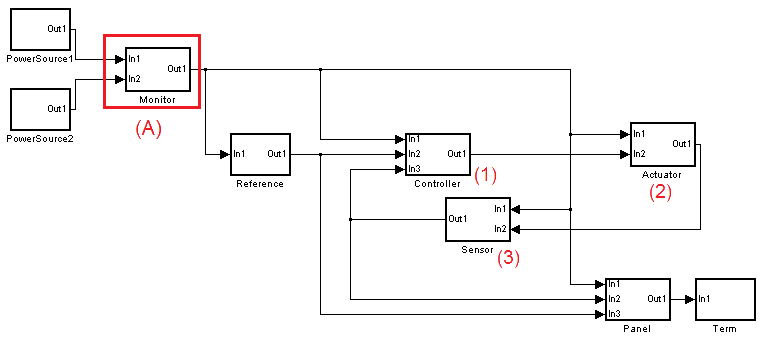
\includegraphics[width=\linewidth]{acsBlockDiagrams}
\end{frame}

\begin{frame}
\frametitle{Fault Tolerance, Failure Logic, Safety Analysis}
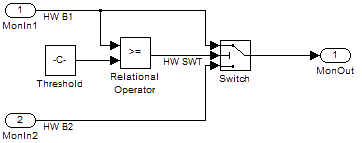
\includegraphics[height=0.4\textheight]{blockDiagramMonitorInternals}\par
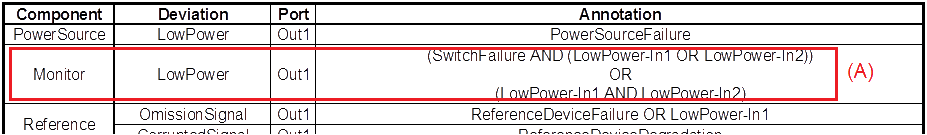
\includegraphics[width=\linewidth]{acsAnnotations}
\end{frame}

\begin{frame}[fragile]
\frametitle{\CSPM to inject faults and obtain fault traces}
From:\\
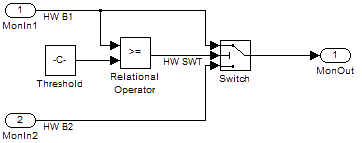
\includegraphics[height=0.3\textheight]{blockDiagramMonitorInternals}\par

We obtain traces with faults:
{\tiny
\begin{itemize}
  \item \verb|failure.Hardware.N04_RelationalOperator| -- HW SWT \onslide<2->{(S)}
  \item \verb|failure.Hardware.N04_MonIn1| -- HW B1 \onslide<2->{(A)}
  \item \verb|failure.Hardware.N04_MonIn2| -- HW B2 \onslide<2->{(B)}
\end{itemize}
}

\end{frame}

\begin{frame}[fragile]
\frametitle{Faults trace example}
Two of the 64 traces are:
\begin{snippetcspm}[0]
TRACE 1:
failure.Hardware.N04_MonIn2.1.EXP.I.5
failure.Hardware.N04_MonIn2.1.ACT.OMISSION
failure.Hardware.N04_RelationalOperator.1.EXP.B.true
failure.Hardware.N04_RelationalOperator.1.ACT.B.false
out.1.OMISSION

TRACE 2:
failure.Hardware.N04_MonIn1.1.EXP.I.5
failure.Hardware.N04_MonIn1.1.ACT.OMISSION
failure.Hardware.N04_MonIn2.1.EXP.I.5
failure.Hardware.N04_MonIn2.1.ACT.OMISSION
out.1.OMISSION
\end{snippetcspm}
\footnotesize
\begin{itemize}
  \item Combine each trace with conjunctions: $B \land S$, $A \land B$, \ldots
  \item Combine all traces with disjunctions: $(B \land S) \lor (A \land B) \lor \ldots$
  \item The complete failure logic after simplification is exactly the supplied by Embraer: \alert<4>{$(A \land B) \lor (S \land (A \lor B))$}
  \item <2-> Note that we ignore events order in each trace, because Boolean AND is commutative.
  \item<3-> Some traces appear in a specific order: $A$ then $S$, but not $S$ then $A$.
\end{itemize}

\onslide<4>{\tikzoverlay[text width=3cm] at (3.8cm,2.7cm) {a.k.a structure function or structure expression};}
\end{frame}

\section{Fault Trees}

\subsection{Static Fault Trees}

\begin{frame}
\frametitle{Static Fault Trees}
\begin{tikzpicture}[fault tree, global scale=0.7]
\node (r) [event] {Low Power}
    child {
      node (both) [event] {Both inputs fail}
      child { node (a1) [event] {A fails} } 
      child { node (b1) [event] {B fails} }
    }
    child {
      node (si) [event] {One input fails and the switcher fails}
      child { node (s) [event] {Switcher fails}}
      child { 
        node (oneinput) [event] {One input fails}
        child { node (a2) [event] {A fails} }
        child { node (b2) [event] {B fails} }
      }
    };

\node [or gate] (or1) at (r.south) {};
\node [and gate] (and1) at (both.south) {};
\node [and gate] at (si.south) {};
\node [or gate] at (oneinput.south) {};
\node [basic] at (a1.south) {};
\node [basic] at (a2.south) {};
\node [basic] at (b1.south) {};
\node [basic] at (b2.south) {};

\onslide<2->{
\node (rdescr) [above right=0.5cm and 0cm of r] {Root event};
\draw (rdescr) edge[->] (r);

\node (interdescr) [above right=0.5cm and 0cm of si] {Intermediary event};
\draw (interdescr) edge[->] (si);

\node (ordescr) [below right=0 and 0.5cm of or1] {OR gate};
\draw (ordescr) edge[->] (or1);

\node (anddescr) [below right=0 and 0.5cm of and1] {AND gate};
\draw (anddescr) edge[->] (and1);

\node (basicdescr) [below right=0.3 and 0.5cm of a1] {Basic event};
\draw (basicdescr) edge[->] (a1);
}

      %child {
      %  node [and gate] {}
      %  child {
      %    node [event] {One input fails and the switcher fails}
      %    child { node [basic] {Switcher fails} }
      %    child {
      %      node [event] {One input fails}
      %      child {
      %        node [or gate] {}
      %        child [basic] {A fails}
      %        child [basic] {B fails}
      %      }
      %    }
      %  }
      %}
\end{tikzpicture}
\end{frame}

\subsection{Dynamic Fault Trees}

\begin{frame}
\frametitle{Dynamic Fault Trees}
\begin{itemize}
  \item Priority AND -- PAND\\
    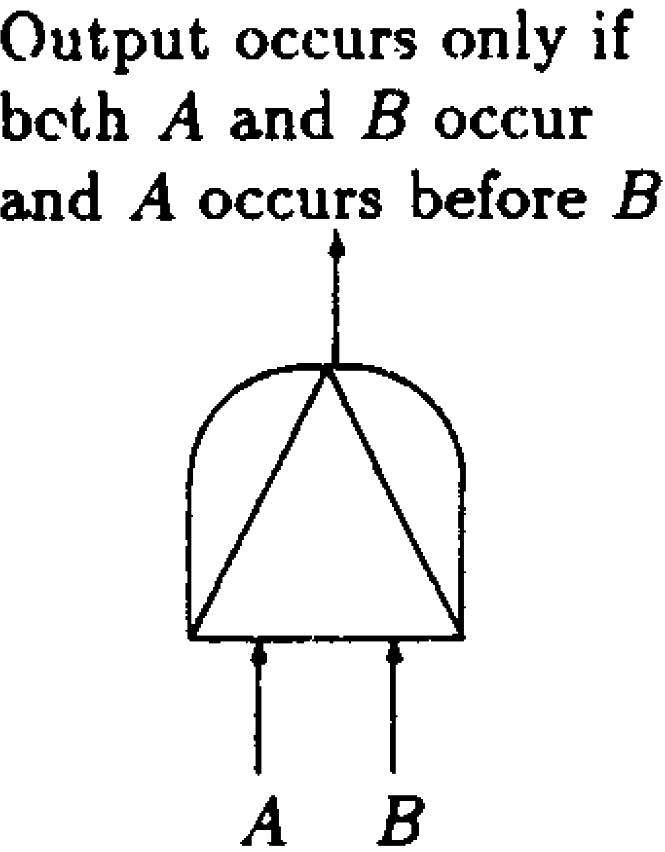
\includegraphics[height=4cm]{pand-dugan}
\end{itemize}
\end{frame}

\begin{frame}
\frametitle{Dynamic Fault Trees}
\begin{itemize}
  \item Cold Spare gate -- CSP\\
    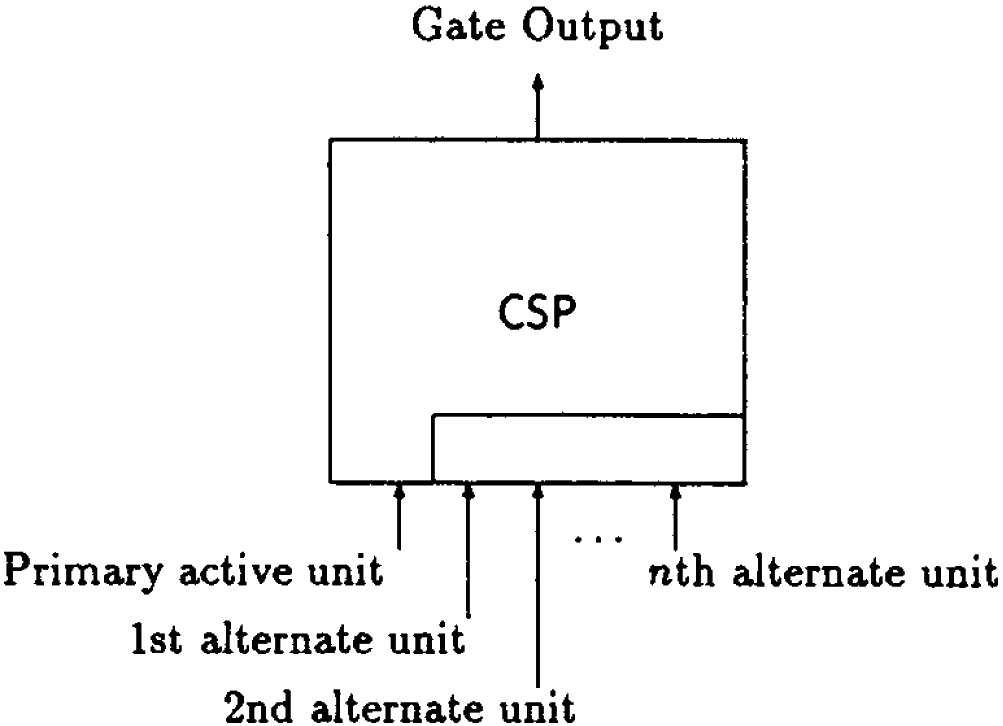
\includegraphics[height=4cm]{csp-dugan}
  \item Example: 4 tires, 1 spare
\end{itemize}
\end{frame}

\begin{frame}
\frametitle{Dynamic Fault Trees}
\begin{itemize}
  \item Sequence Enforcing gate -- SEQ (dummy output)\\
    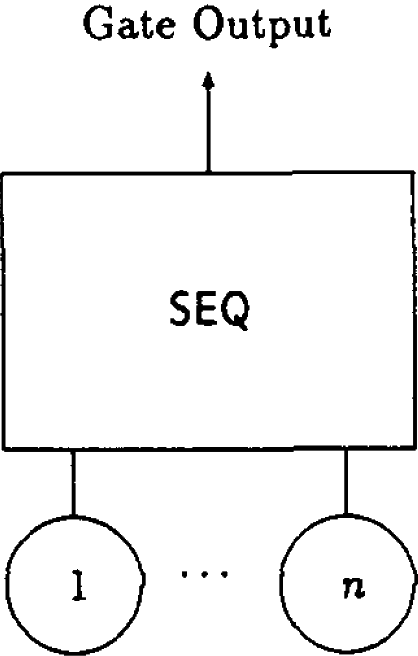
\includegraphics[height=4cm]{seq-dugan} 
  \item Events are forced to occur in a specific order
\end{itemize}
\end{frame}

\begin{frame}
\frametitle{Dynamic Fault Trees}
\begin{itemize}
  \item Functional Dependency gate -- FDEP (dummy output)\\
    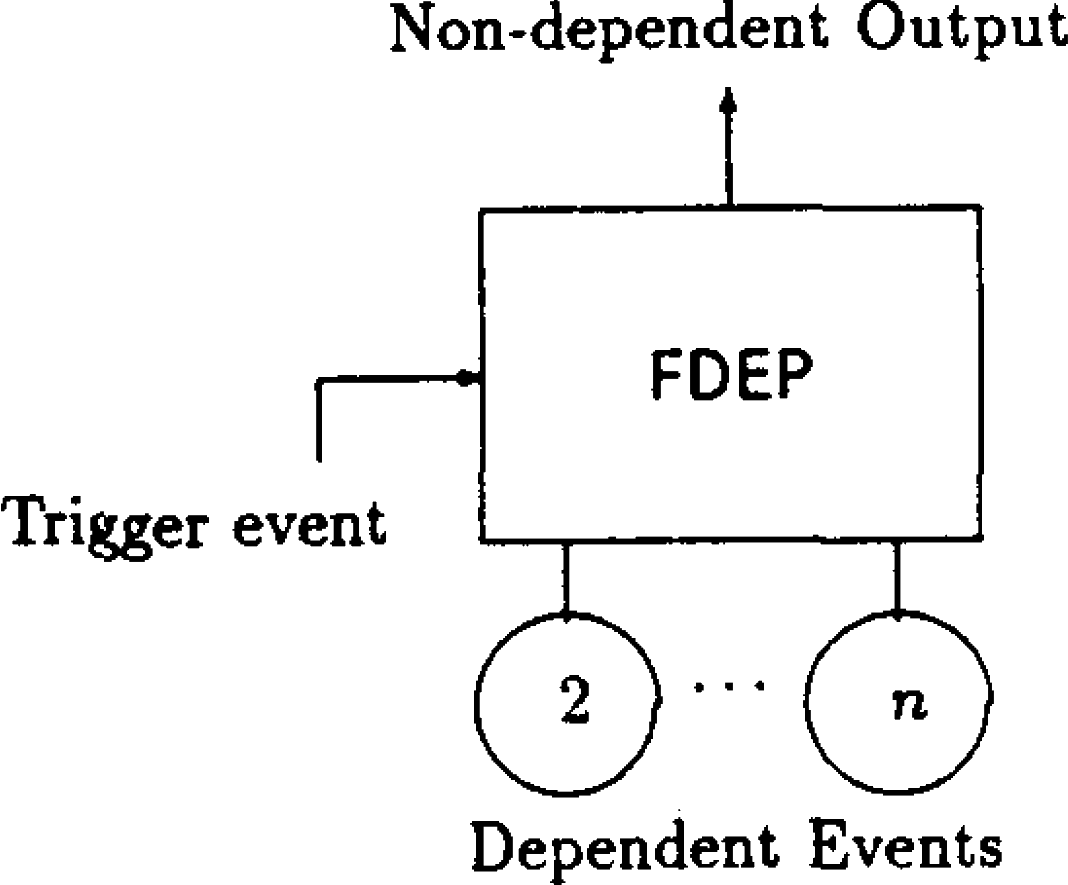
\includegraphics[height=4cm]{fdep-dugan}
  \item Dependent events are forced to occur when the trigger events activates;
  \item Otherwise they are independent.
\end{itemize}
\end{frame}

\begin{frame}
\frametitle{Relevant DFT gates}
\begin{itemize}
  \item SEQ is expressible in terms of CSP.
  \item For DFT, the relevant gates are then PAND, FDEP and CSP. 
\end{itemize}
\end{frame}

\subsection{Temporal Fault Trees}

\begin{frame}
\frametitle{Temporal Fault Trees}
\begin{itemize}
  \item Priority AND gate -- PAND\\
  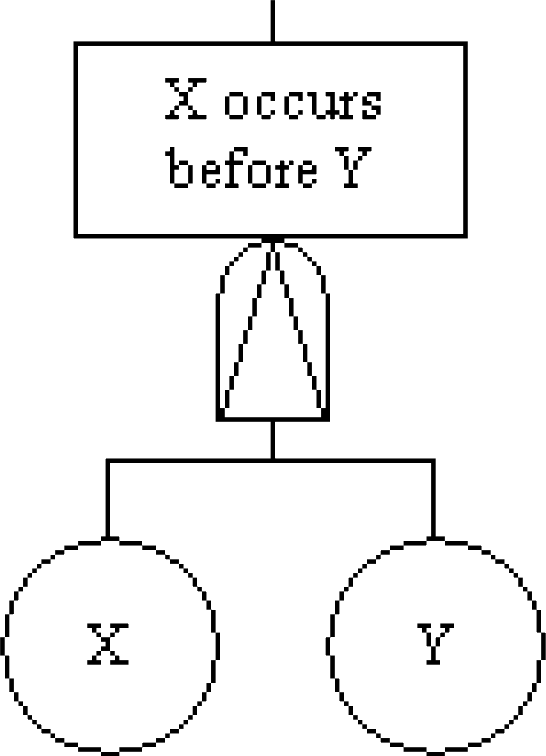
\includegraphics[height=4cm]{pand-walker}
\end{itemize}
\end{frame}

\begin{frame}
\frametitle{Temporal Fault Trees}
\begin{itemize}
  \item Priority OR gate -- POR\\
  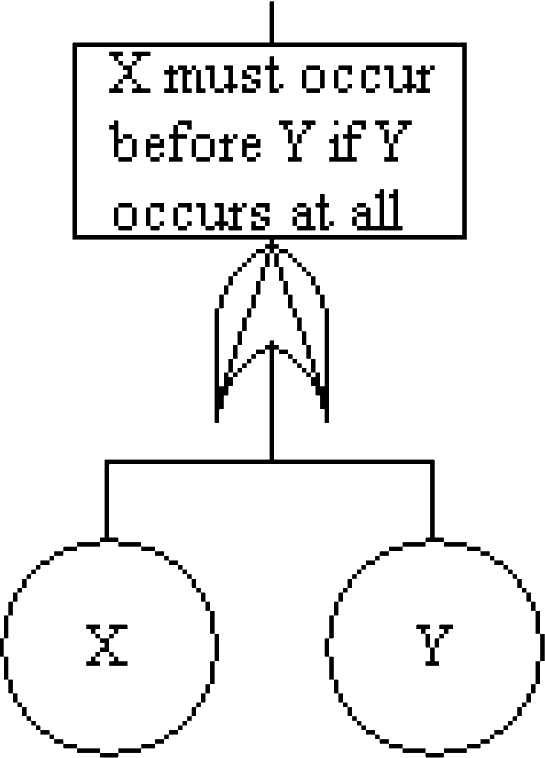
\includegraphics[height=4cm]{por-walker}
\end{itemize}
\end{frame}

\begin{frame}
\frametitle{Temporal Fault Trees}
\begin{itemize}
  \item Simultaneous gate -- SAND\\
  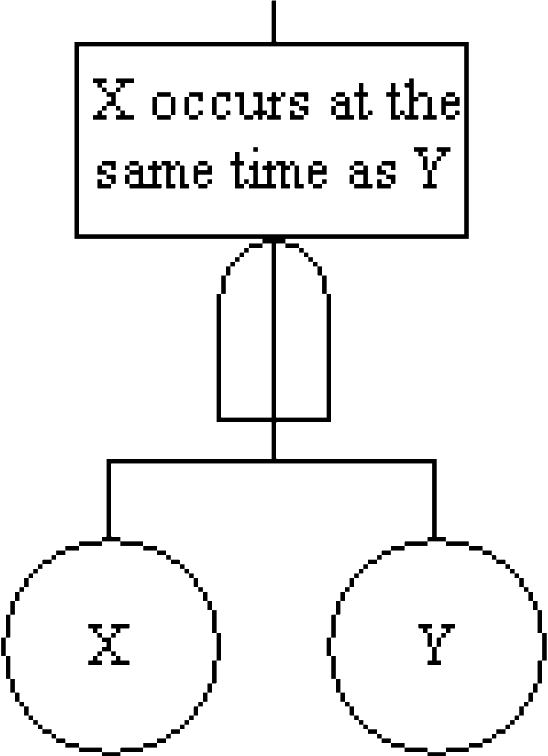
\includegraphics[height=4cm]{sand-walker}
\end{itemize}
\end{frame}





\begin{frame}
\frametitle{Fault modelling and safety design patterns}
\begin{itemize}
  \item Faults injection to find failures---it's an important approach to discover hidden faults combination;
  \item Fault modelling is a more detailed approach, to let a designer model nominal behaviour and erroneous behaviour at the same time.
  \item Two approaches analyse system safety: fault injection and fault modelling 
\end{itemize}
\end{frame}

\begin{frame}[fragile]
\frametitle{Analyse system safety with fault injection}

\begin{itemize}
  \item From traces
\begin{snippetcspm}[0]
TRACE 1:
failure.Hardware.N04_MonIn2.1.EXP.I.5
failure.Hardware.N04_MonIn2.1.ACT.OMISSION
failure.Hardware.N04_RelationalOperator.1.EXP.B.true
failure.Hardware.N04_RelationalOperator.1.ACT.B.false
out.1.OMISSION

TRACE 2:
failure.Hardware.N04_MonIn1.1.EXP.I.5
failure.Hardware.N04_MonIn1.1.ACT.OMISSION
failure.Hardware.N04_MonIn2.1.EXP.I.5
failure.Hardware.N04_MonIn2.1.ACT.OMISSION
out.1.OMISSION
\end{snippetcspm}
  \item We obtain \emph{lists} $[B,S]$, $[A,B]$---a finite set of lists
  \item We need an algebra to reduce the set of lists 
\end{itemize}
\end{frame}

\begin{frame}
\frametitle{Inspiration: Free Boolean Algebra}
\begin{itemize}
  \item Free variables: A, B, C, \ldots
  \item Any Boolean formula in Free Boolean Algebra (FBA) is written as a set of sets
    \begin{itemize}
      \item For an algebra with three variables $\{A,B,C\}$
      \item $A \lor B =_{\fba} \{ \{A\}, \{B\}, \{A,B\}  \}$
      \item $\lnot A =_{\fba} \{ \{\,\}, \{B\},\{C\},\{B,C\}  \} $
    \end{itemize}  
  \item In Isabelle/HOL, the AFP has a theory to formalize FBAs
  \item An inductive set ($\fba$) defines a set of all possible formulas

\end{itemize}
\end{frame}

\begin{frame}
\frametitle{Free Boolean Algebra}
Given the inductive set $\fba$
\begin{subequations}
\begin{align}
\{F | i \in F \} & \in \fba & \text{(Variable)}\\
S \in \fba \implies -S & \in \fba & \text{(Complement)}\\
S \in \fba \land T \in \fba \implies S \inter T & \in \fba & \text{(Intersection)}
\end{align}
\end{subequations}

The Boolean algebra elements ($\top$, $\bot$) and operators ($\lor$, $\land$, $\lnot$) are defined:
\begin{itemize}
  \item $\top =_{\fba} UNIV$ (all sets of free variables combinations)
  \item $\bot =_{\fba} \{\}$
  \item $A =_{\fba} \{F | A \in F\} $
  \item $A \land B =_{\fba} \{F | A \in F \} \inter \{F | B \in F\}$ 
  \item $A \lor B =_{\fba} \{F | A \in F \} \union \{F | B \in F\}$
  \item $\lnot A =_{\fba} - \{F | A \in F\}$
\end{itemize}
\end{frame}

\begin{frame}
\frametitle{Temporal Faults Algebra}

\begin{itemize}
  \item Free Variables
  \item Any formula is written as a set of lists
    \begin{itemize}
      \item For an algebra with three variables $\{A,B,C\}$
      \item $A \lor B =_{\tfa} \{ [A], [B], [A,B], [B,A], [A,B,C], [A,C,B], \ldots, [C,B,A]  \}$
      \item $\lnot A =_{\tfa} \{ [\,], [B], [C], [B,C], [C,B] \} $
      \item $A \xbefore B =_{\tfa} \{ [A,B] \}$
    \end{itemize}  
  \item An inductive set ($\tfa$) defines a set of all possible formulas
\end{itemize}
\end{frame}

\begin{frame}
\frametitle{Temporal Faults Algebra}

$\tvar x = \{l | \distinct l \land x \in \set l\}$
%
\begin{subequations}
\begin{align}
%
\tvar x &\in \tfa & \text{Variable}\\
%
S \in \tfa \implies \{ l | l \in -S \land \distinct l\} &\in \tfa & \text{Negation}\\
%
S \in \tfa \land T \in \tfa \implies 
S \inter T &\in \tfa & \text{Intersection} \\
%
S \in \tfa \land T \in \tfa \implies 
S \rightarrow T & \in \tfa & \text{Exclusive before }
%
\end{align} %
%
\end{subequations}%

The Boolean algebra elements ($\top$, $\bot$) and operators ($\lor$, $\land$, $\lnot$) are defined:
\begin{itemize}
  \item $\top =_{\tfa} \{l | \distinct l\}$ (all sets of distinct lists)
  \item $\bot =_{\tfa} \{\}$
  \item $A =_{\tfa} \tvar A $
  \item $A \land B =_{\tfa} \tvar A \inter \tvar B$
  \item $A \lor B =_{\tfa} \tvar A \union \tvar B$
  \item $\lnot A =_{\tfa} \{l | l \in - \tvar A \land \distinct l\}$
\end{itemize}
\end{frame}

\begin{frame}{Exclusive before definition}
\begin{align*}
S \rightarrow T = &\left\{ l \bullet \exists xs, ys | xs \in (S - T) \land ys \in (T - S) \land \right.
%
\\& \left. distinct (xs \concat ys) \land l = xs \concat ys \right\}
\end{align*}

Example:
\begin{align*}
\tvar a =& \left\{[a],[a,b],[b,a],[a,c],[c,a],[a,b,c],\ldots,[c,b,a]\right\} \\
\tvar b =& \left\{[b],[a,b],[b,a],[b,c],[c,b],[a,b,c],\ldots,[c,b,a]\right\} \\
\tvar a \rightarrow \tvar b =& \left\{[a,b],[a,b,c],[a,c,b],[c,a,b]\right\}
\end{align*}

\end{frame}

\begin{frame}
\frametitle{Temporal Faults Algebra -- Isabelle/HOL}
\includeautosizegraphics{tformula-01}

\onslide<2>{%
\tikzoverlay[text width=6.5cm] at (4.5cm,5.5cm) {%
$a \tformulat = tfa :: a \listt \sett \sett $\\
$Abs\_\tformulat :: a \listt \sett \sett \Rightarrow a \tformulat $\\ 
$Rep\_\tformulat :: a \tformulat \Rightarrow a \listt \sett \sett $%
};
}
\end{frame}

\begin{frame}
\frametitle{Temporal Faults Algebra -- Isabelle/HOL}
\includeautosizegraphics{tformula-02}
\end{frame}

\begin{frame}
\frametitle{Safety analysis using structure function}

\begin{itemize}
  \item Qualitative analysis:
    \begin{itemize}
      \item Obtaining minimal cut sets -- sets of events that cause the top fault event \onslide<2->{-- Rule: \alert<2>{$\BasicEventMinLevel$}}
      \item Importance analysis -- cut sets with fewer events are more important
      \item Minimal cut sets susceptible to common cause failures
    \end{itemize}
  \item Quantitative analysis:
    \begin{itemize}
      \item Absolute probability of the top event \onslide<2->{-- Rule: \alert<3>{$\RootProbability$}}
      \item Quantitative component importance -- percentage of time that a system failure is caused by a particular minimal cut set
      \item Effects of changing maintenance and checking time, implementing design modifications or changing component reliabilities
    \end{itemize}
\end{itemize}
\end{frame}

\begin{frame}
\frametitle{Fault Tree Rule evaluation (or acceptance criteria)}


Function $\evaluateRule$ is defined as:
$\evaluateRule :: FaultTree \Rightarrow FaultTreeRule \Rightarrow Probability \Rightarrow bool$
{
\footnotesize 
\begin{subequations}
\begin{align}
\evaluateRule ft \, (\BasicEventMinLevel n) P &= (\minBasicEventLevel ft \ge n)\\
\evaluateRule ft \, (\RootProbability p) P &= (\ftProbability ft \, P) \le p
\end{align}
\end{subequations}
}

Function $\minBasicEventLevel$ is defined as $0$ if the structure expression is a variable or $1$ plus the minimum of $\minBasicEventLevel$ of the subexpressions.
%
Function $\ftProbability$ calculates the probability of an expression, given the probability of basic events (variables). Ex.: $\ftProbability (A \lor B) P = P(A) + P(B) - P(A) \times P(B)$
\end{frame}

\begin{frame}
\frametitle{Fault modelling}

\begin{itemize}
  \item By component. Ex.: if fault $\failurevalue{A}{1}$ occurs in some component $\component{1}$, the output is $\outvalue{U}{1}$, if fault $\failurevalue{B}{1}$ occurs, the output is $\outvalue{V}{1}$, otherwise, the output is nominal.
  \item Interface-focused. Ex.: if component $\component{2}$ is connected in its input port $1$ to component $\component{1}$, then if $\component{2}$ observes some fault $\failurevalue{A}{1}$ in input port $1$ caused by $\component{1}$, then $\component{2}$ output is $\outvalue{U}{2}$, otherwise the output is nominal.
\end{itemize}

\end{frame}

\begin{frame}
\frametitle{Activation Algebra for fault modelling}
\begin{itemize}
  \item Faults are variables in some algebra ($\failurevalue{A}{1} = \failurevalue{\text{Internal failure}}{1}$, $\failurevalue{A}{2}=\failurevalue{\text{Internal failure}}{2}$)
  \item Each operand is a pair: (i) an expression in some algebra (Boolean or Temporal), and (ii) an output value.
  \item Output values are identified by: (i) a failure mode and optionally a numerical value (ex.: $\outvalue{U}{1}$ = Omission), or (ii) $N$ and a numerical value to express a nominal value. 
  \item Ex.: $exp = \aaexp{\alert<2>{\failurevalue{A}{1}}}{\alert<4>{\outvalue{U}{1}}} \alert<2>{\lor} \aaexp{\alert<2>{\lnot \failurevalue{A}{1}}}{\nominalvalue{5}{1}}$
  \item<2-> The expressions of the algebra when combined should give a tautology: $\failurevalue{A}{1} \lor \lnot \failurevalue{A}{1} = \top$
  \item<3-> Predicate:
  $P\left(exp\right) \defs \alert<4>{\outvalueof{exp}=\outvalue{U}{1}} \iff 
  %
  P\left(exp\right) = \failurevalue{A}{1}$
  \item<4-> We then use the predicates in the given algebra to apply Fault Tree Rules
\end{itemize}
\end{frame}

\begin{frame}[fragile]
\frametitle{Activation Algebra for our example}

\begin{itemize}
  \item $\failurevalue{S}{1}$: SwitchFailure
  \item $\failurevalue{A}{1}$: LowPower in input 1
  \item $\failurevalue{B}{1}$: LowPower in input 2
  \item $\failurevalue{L}{1}$: LowPower in $\component{1}$
  \item $out_1 = 
  \aaexp{\failurevalue{A}{1} \land \failurevalue{B}{1}}{\failurevalue{L}{1}} \lor
  \aaexp{\failurevalue{S}{1} \land (\failurevalue{A}{1} \lor \failurevalue{B}{1})}{\failurevalue{L}{1}} \lor
  \aaexp{\lnot A \lor \lnot B}{\nominalvalue{12}{1}} \lor
  \aaexp{\lnot S \lor (\lnot A \land \lnot B)}{\nominalvalue{12}{1}}
  $
  \item $P_1\left(out_1\right) \defs \outvalueof{out_1}=\failurevalue{L}{1}$
  \item<2-> $P_1\left(out_1\right) = \left(\failurevalue{A}{1} \land \failurevalue{B}{1}\right) \lor 
  \left(\failurevalue{S}{1} \land \left(\failurevalue{A}{1} \lor \failurevalue{B}{2}\right)\right)$
\end{itemize}
\end{frame}

\begin{frame}[fragile]{Progress analysis}
  \begin{columns}
    \begin{column}{0.45\paperwidth}
        \begin{itemize}
          \item<1-> Connect to TFA
          \item<2-> Write in activation algebra notation
          \item<3-> Rewrite with new TFA definitions
          \item<4-> TFA laws are only applied to variables on Merle's algebra
          \item<5-> Reduce TFA automatically -- use of trees like in FBA
          \item<6-> Verification of criteria in TFA expressions is still an issue and dependes on TFA's reduction
          \item<7-> Suggest model changes after FT criteria verification
        \end{itemize}
    \end{column}
    \begin{column}{0.45\paperwidth}
        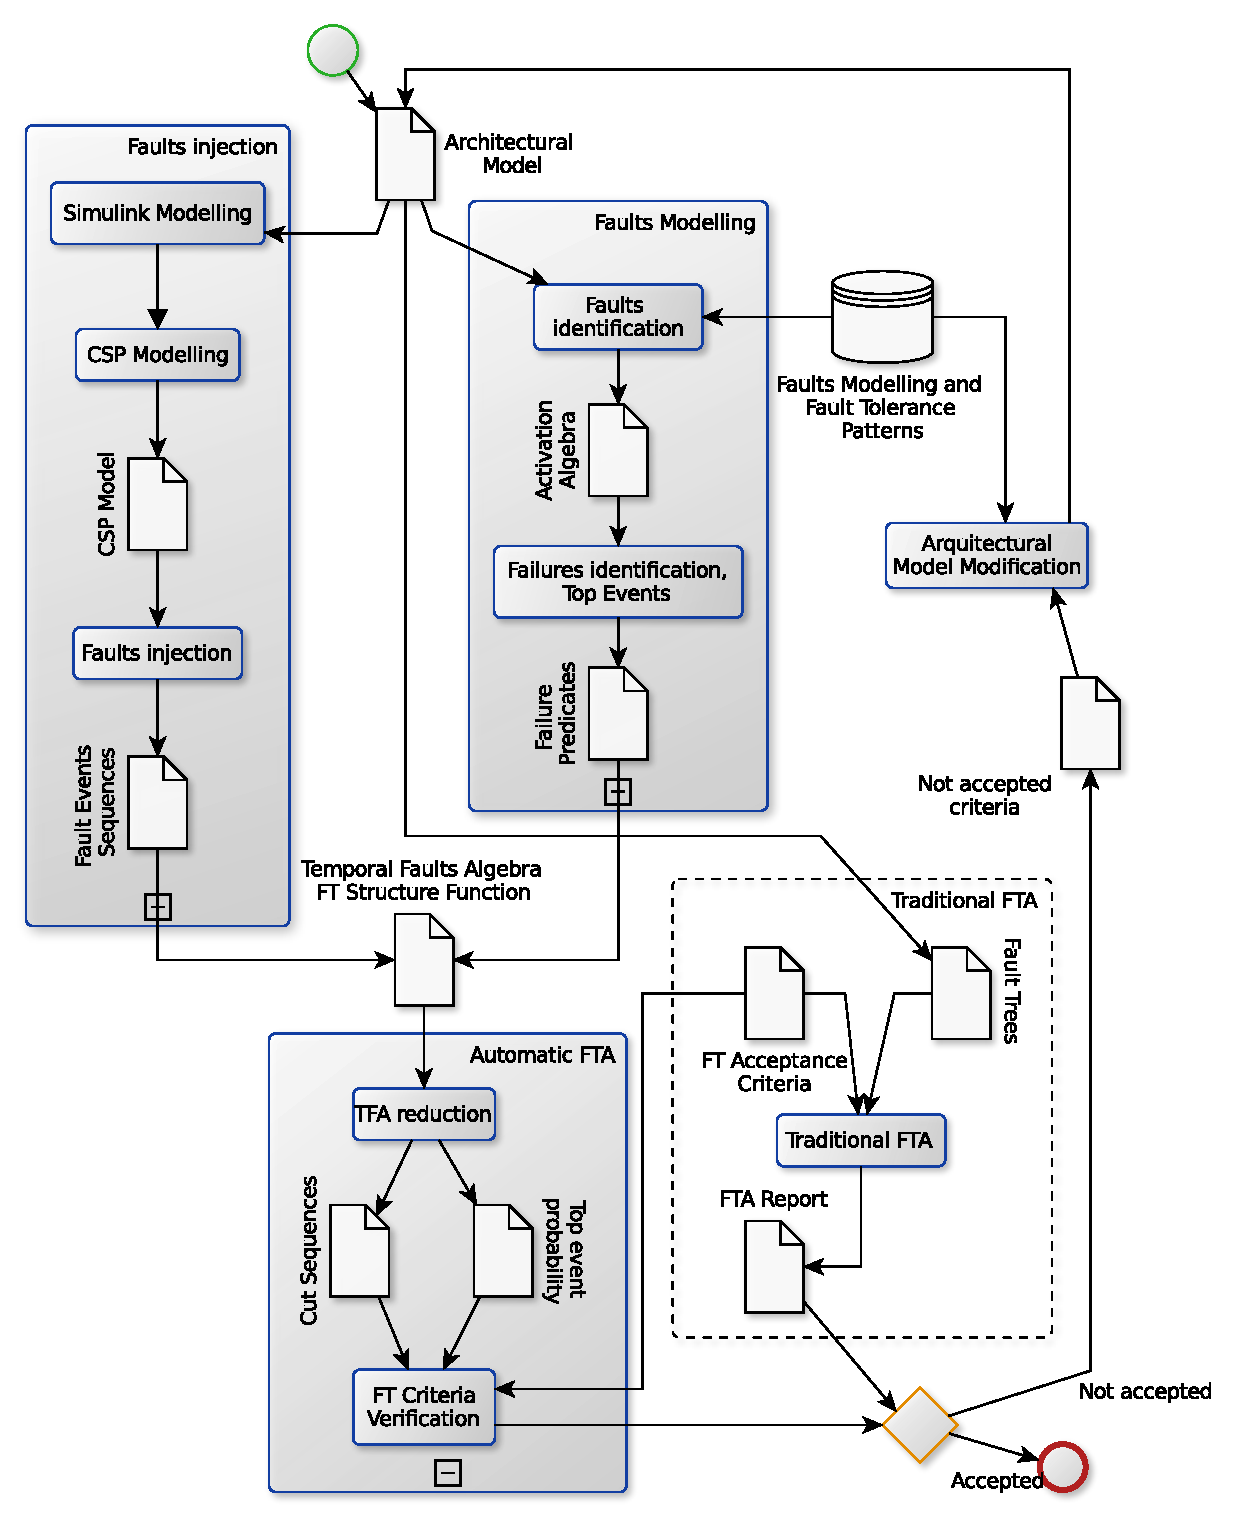
\includegraphics[width=\textwidth]{StrategyOverview}
        \begin{tikzpicture}[overlay, progress/.style={font=\huge}]
        \node<1->[progress] (v1) at (-0.1,24) {90\%};
        \node<2->[progress] (v2) at (9.6,18.2) {0\%};
        \node<3->[progress] (v3) at (8.1,22.5) {75\%};
        \node<4->[progress] (v4) at (0,10.5) {50\%};
        \node<5->[progress] (v5) at (3.4,7.0) {20\%};
        \node<6->[progress] (v6) at (3.5,1.4) {20\%};
        \node<7->[progress] (v7) at (10.8,15.5) {0\%};
        \end{tikzpicture}
    \end{column}
\end{columns}


\end{frame}



\end{document}
